
\begin{figure}[H]
  {
    \setlength{\tabcolsep}{3.0pt}
    \setlength\cmidrulewidth{\heavyrulewidth} % Make cmidrule = 
    \begin{adjustbox}{height=5cm,center}
      \footnotesize
      \begin{tabular}{ll}

        \makecell[l]{
\icode{.BYTE \$00,\$00,\$00,\$FF,\$FE,\$FD,\$01,\$02}\\
\icode{.BYTE \$00,\$FF,\$FE,\$01,\$02,\$03,\$01,\$02}
} & \makecell[l]{
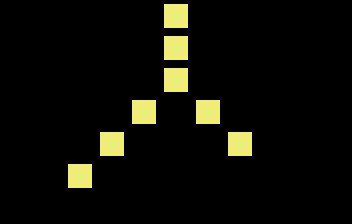
\includegraphics[width=1.3cm]{src/patterns/pixels/pixel_pattern8_0.png}%
} \\
        \midrule

        \makecell[l]{
\icode{.BYTE \$00,\$03}\\
\icode{.BYTE \$00,\$03}
} & \makecell[l]{
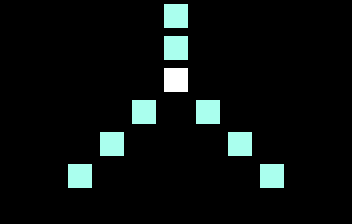
\includegraphics[width=1.3cm]{src/patterns/pixels/pixel_pattern8_1.png}%
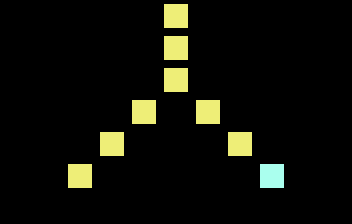
\includegraphics[width=1.3cm]{src/patterns/pixels/pixel_pattern8_2.png}%
} \\
        \midrule

        \makecell[l]{
\icode{.BYTE \$00,\$00,\$00,\$00,\$00}\\
\icode{.BYTE \$00,\$01,\$02,\$03,\$04}
} & \makecell[l]{
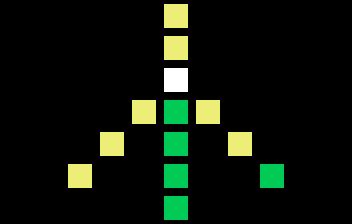
\includegraphics[width=1.3cm]{src/patterns/pixels/pixel_pattern8_3.png}%
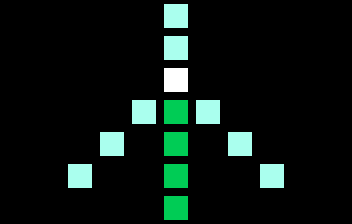
\includegraphics[width=1.3cm]{src/patterns/pixels/pixel_pattern8_4.png}%
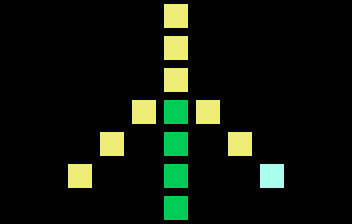
\includegraphics[width=1.3cm]{src/patterns/pixels/pixel_pattern8_5.png}%
} \\
        \midrule

        \makecell[l]{
\icode{.BYTE \$00,\$FF,\$FE,\$FC,\$FB,\$FC,\$01,\$02}\\
\icode{.BYTE \$00,\$FE,\$FE,\$FF,\$01,\$03,\$FE,\$FE}
} & \makecell[l]{
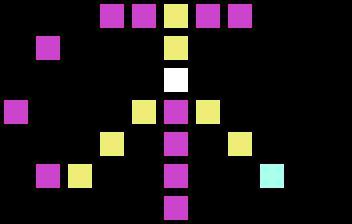
\includegraphics[width=1.3cm]{src/patterns/pixels/pixel_pattern8_6.png}%
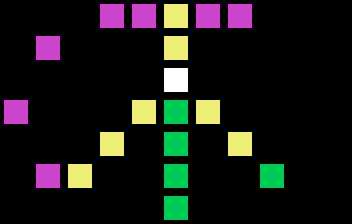
\includegraphics[width=1.3cm]{src/patterns/pixels/pixel_pattern8_7.png}%
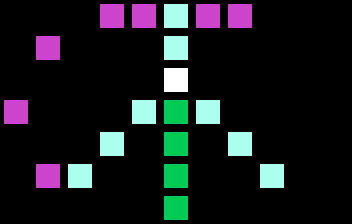
\includegraphics[width=1.3cm]{src/patterns/pixels/pixel_pattern8_8.png}%
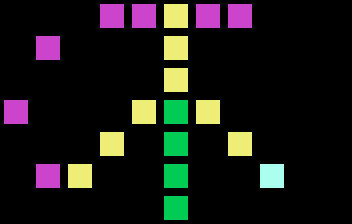
\includegraphics[width=1.3cm]{src/patterns/pixels/pixel_pattern8_9.png}%
} \\
        \midrule

        \makecell[l]{
\icode{.BYTE \$00,\$04,\$05,\$04,\$FF,\$01}\\
\icode{.BYTE \$00,\$FF,\$01,\$03,\$04,\$04}
} & \makecell[l]{
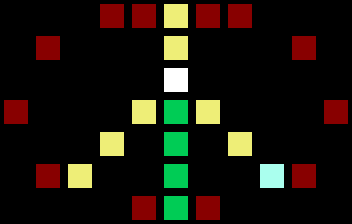
\includegraphics[width=1.3cm]{src/patterns/pixels/pixel_pattern8_10.png}%
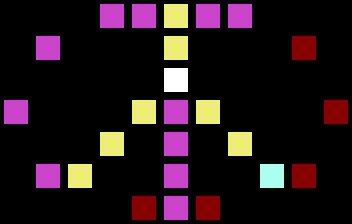
\includegraphics[width=1.3cm]{src/patterns/pixels/pixel_pattern8_11.png}%
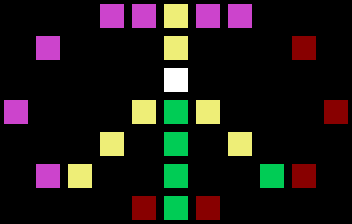
\includegraphics[width=1.3cm]{src/patterns/pixels/pixel_pattern8_12.png}%
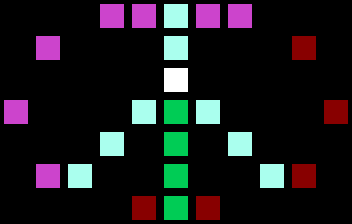
\includegraphics[width=1.3cm]{src/patterns/pixels/pixel_pattern8_13.png}%
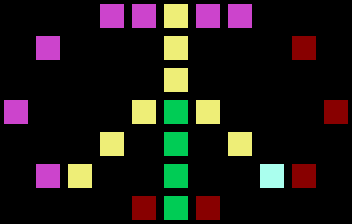
\includegraphics[width=1.3cm]{src/patterns/pixels/pixel_pattern8_14.png}%
} \\
        \midrule

        \makecell[l]{
\icode{.BYTE \$00,\$FD,\$FB,\$03,\$05,\$02,\$FE}\\
\icode{.BYTE \$00,\$FF,\$00,\$FF,\$00,\$04,\$04}
} & \makecell[l]{
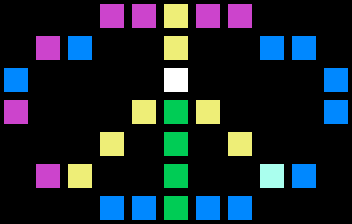
\includegraphics[width=1.3cm]{src/patterns/pixels/pixel_pattern8_15.png}%
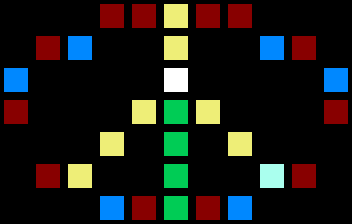
\includegraphics[width=1.3cm]{src/patterns/pixels/pixel_pattern8_16.png}%
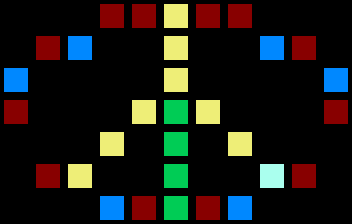
\includegraphics[width=1.3cm]{src/patterns/pixels/pixel_pattern8_17.png}%
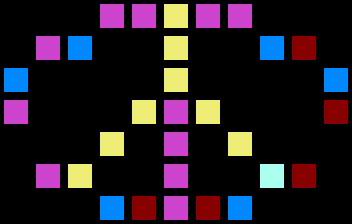
\includegraphics[width=1.3cm]{src/patterns/pixels/pixel_pattern8_18.png}%
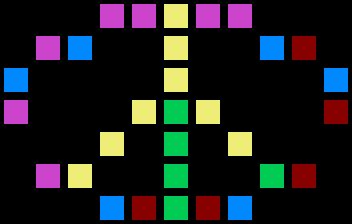
\includegraphics[width=1.3cm]{src/patterns/pixels/pixel_pattern8_19.png}%
} \\
        \midrule

        \makecell[l]{
\icode{.BYTE \$00}\\
\icode{.BYTE \$00}
} & \makecell[l]{
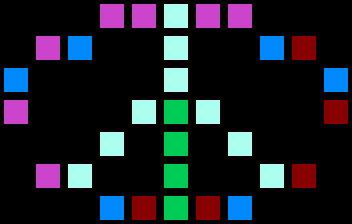
\includegraphics[width=1.3cm]{src/patterns/pixels/pixel_pattern8_20.png}%
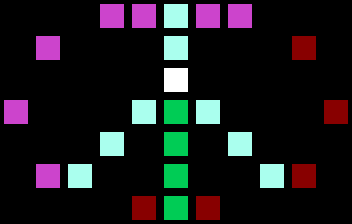
\includegraphics[width=1.3cm]{src/patterns/pixels/pixel_pattern8_21.png}%
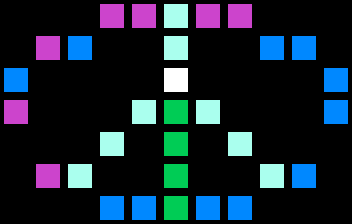
\includegraphics[width=1.3cm]{src/patterns/pixels/pixel_pattern8_22.png}%
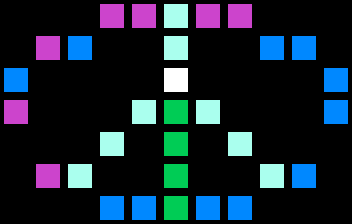
\includegraphics[width=1.3cm]{src/patterns/pixels/pixel_pattern8_23.png}%
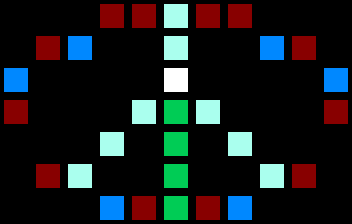
\includegraphics[width=1.3cm]{src/patterns/pixels/pixel_pattern8_24.png}%
} \\
        \midrule

      \end{tabular}
    \end{adjustbox}
  }\caption{The purpose of each of the oscillator values.}
\end{figure}
